\documentclass[a4paper,12pt]{article}

\usepackage{amsfonts}
\usepackage{amsmath}
\usepackage{float}
\usepackage{graphicx}
\usepackage{listings}
\usepackage[margin=1in]{geometry}

\title{Assignment 3: Applications of Image Processing to Real-World Problems}
\author{Aleksandr Jan Smoliakov}
\date{2024--12--20}

\begin{document}

\maketitle

\section{Introduction}

The report is structured into three sections, each of which describes a different application of image processing to a real-world problem.

In \textbf{FISH Signal Counts}, we analyze fluorescence in situ hybridization (FISH) images to detect and quantify genetic mutations in tumor cells. This involves identifying mutations using fluorescent probes and quantifying the signals to understand the mutation distribution within individual cells.

In \textbf{Circuit Board Quality Assurance}, we analyze images of circuit boards to detect defects. This involves inspecting soldering regions, traces, and drilled holes using x-ray imaging and image processing techniques.

In \textbf{Filled Bottles}, we analyze images of a production line to detect whether bottles are filled to the correct level. This involves detecting the liquid level in bottles using edge detection and intensity analysis.

\newpage

\tableofcontents

\newpage

\section{Theoretical Background}

Understanding the real-world applications described in the next sections of this report requires familiarity with several key concepts in digital image processing. This section provides a brief overview of these concepts, namely colour fundamentals, thresholding, morphological operations, image segmentation, and connected components labeling.

\subsection{Thresholding}

Thresholding is a fundamental technique in digital image analysis used to separate objects of interest from the background. The process assigns a binary label to each pixel based on a predefined intensity level called the \emph{threshold}. Mathematically, for a grayscale image \(f(x, y)\) and a threshold \(T\), the thresholded image \(g(x, y)\) can be expressed as:

\[
g(x, y) = 
\begin{cases}
1, & \text{if } f(x, y) \geq T, \\
0, & \text{otherwise}.
\end{cases}
\]

Here, \(g(x, y)\) is referred to as a \emph{binary} image, where \(1\) typically denotes foreground (e.g. object of interest) and \(0\) denotes background. Depending on the application, the foreground can represent different elements (e.g. cells in a microscopy image or elements in a circuit board).

This technique can be extended to \emph{multiple thresholding} where more than two classes are defined based on different intensity ranges. Mathematically, for \(n\) thresholds \(T_1, T_2, \ldots, T_n\), the thresholded image \(g(x, y)\) can be expressed as:

\[
g(x, y) =
\begin{cases}
1, & \text{if } f(x, y) \geq T_n, \\
\vdots & \\
n, & \text{if } T_{n-1} \leq f(x, y) < T_n, \\
0, & \text{otherwise}.
\end{cases}
\]

However, in the subsequent sections, we focus on the basic binary thresholding technique for simplicity and clarity.

\subsubsection{Basic Global Thresholding}

The simplest form of thresholding assumes a single, constant threshold \(T\) that partitions the image into two classes (background and foreground). To determine this threshold, one can examine the intensity histogram of the image. A straightforward approach is to choose \(T\) as the \emph{midpoint} between the average foreground and average background intensities, or use domain-specific heuristics.

An improved version of basic global thresholding involves iterative selection:
\begin{enumerate}
    \item Select an initial estimate for the global threshold \(T\).
    \item Segment the image into background and foreground using \(T\).
    \item Compute the mean intensities \(\mu_b\) and \(\mu_f\) of the background and foreground classes, respectively.
    \item Update \(T \leftarrow \frac{\mu_b + \mu_f}{2}\).
    \item Repeat until \(T\) converges (i.e. the change \(\Delta T\) is below a predefined threshold).
\end{enumerate}

Although this method is simple, it often performs adequately if the intensity histogram is bimodal.

\subsubsection{Optimal Global Thresholding}

The basic global thresholding methods are intuitive but may not be optimal in all scenarios. They can be sensitive to noise, uneven illumination, or complex object-background distributions.

Optimal global thresholding methods aim to find the threshold value \(T\) that best separates the classes in a statistical sense. Typically, this involves maximizing a criterion that quantifies class separability. For instance, one may minimize the overall misclassification error probability by modeling the intensities of the background and foreground with probability density functions (PDFs) and solving for the threshold that minimizes the error.

\subsubsection{Otsu's Method}

Otsu's method is a histogram-based thresholding approach that seeks to maximize the \emph{between-class variance} (or minimize the \emph{within-class variance}) of the thresholded image. Consider an image with an intensity histogram \(p(i)\), where \(i\) ranges over all possible intensity levels \(0 \leq i < L\). For a potential threshold \(T\), define:

\[
\omega_0(T) = \sum_{i=0}^{T-1} p(i), 
\quad
\omega_1(T) = \sum_{i=T}^{L-1} p(i),
\]
\[
\mu_0(T) = \sum_{i=0}^{T-1} i \, p(i) / \omega_0(T), 
\quad
\mu_1(T) = \sum_{i=T}^{L-1} i \, p(i) / \omega_1(T).
\]

The total mean intensity is:
\[
\mu_T = \sum_{i=0}^{L-1} i \, p(i).
\]

The between-class variance \(\sigma_B^2(T)\) is:
\[
\sigma_B^2(T) = \omega_0(T) \left( \mu_0(T) - \mu_T \right)^2 
+ \omega_1(T) \left( \mu_1(T) - \mu_T \right)^2.
\]

Otsu's method exhaustively searches for the threshold \(T^*\) that maximizes \(\sigma_B^2(T)\). This method also performs well when the histogram exhibits clear foreground-background separation.

\subsubsection{Some Considerations for Thresholding}

Thresholding is a popular image segmentation technique because of its simplicity and effectiveness when the foreground and background intensities are well separated. It serves as a preprocessing step for numerous applications, such as object counting in microscopy images, industrial quality control, and document analysis.

By focusing on separating background and foreground, thresholding simplifies more advanced tasks (e.g. morphological operations) and often leads to computational efficiency.

However, as a simple technique, thresholding is sensitive to noise, illumination variations, and complex object-background distributions. For instance, non-uniform lighting can cause regions of the background to appear brighter or darker, leading to incorrect segmentation using a single global threshold. In practice, controlling or normalizing the illumination is often needed. Some common strategies to address these challenges include adaptive thresholding, smoothing, and edge detection.

\subsubsection{Improving Global Thresholding}

One strategy to improve global thresholding is to \emph{smooth} the image before applying the threshold. Common filters include:
\begin{itemize}
    \item \textbf{Gaussian smoothing}: Convolves the image with a Gaussian kernel to reduce high-frequency noise.
    \item \textbf{Median filtering}: Replaces each pixel with the median of its neighborhood.
\end{itemize}

By reducing noise, the histogram becomes less distorted, which typically leads to a clearer separation between the foreground and background intensities.

Another approach is to combine thresholding with edge information. Sharp intensity transitions, identified by edge detection filters (e.g. Sobel), mark the boundaries of objects. Integrating these boundaries helps refine the thresholding result:
\begin{itemize}
    \item \textbf{Post-processing}: After global thresholding, apply edge detection and correct misclassified regions near the edges.
    \item \textbf{Pre-processing}: Use an edge map to guide the selection of local or global thresholds (e.g. adjusting \(T\) in areas with strong edges).
\end{itemize}

\subsubsection{Variable Thresholding}

If the lighting or object intensity is not uniform across the entire image, a single global threshold can be inadequate. One solution is to \emph{partition} the image into subregions and apply a (potentially different) global threshold for each subregion. The subregions can be chosen based on:
\begin{itemize}
    \item \textbf{Regular grids}, i.e. dividing the image into blocks of fixed size.
    \item \textbf{Adaptive segmentation} based on image properties (e.g. intensity gradients).
\end{itemize}

In this strategy, regions with similar illumination conditions can be thresholded more accurately, improving overall segmentation performance.

In \emph{local thresholding}, the threshold at each pixel depends on local image properties, such as the mean or median intensity of its neighborhood. A common approach is to use a weighted sum of the local mean \(\mu_{x,y}\) and standard deviation \(\sigma_{x,y}\), where for each pixel \((x, y)\):

\[
T_{x,y} = a \cdot \sigma_{x,y} + b \cdot \mu_{x,y}.
\]

This allows the threshold to dynamically adapt to changes in illumination across the image. Such methods are especially effective in cases where the intensity varies gradually across the scene.

In summary, thresholding is a cornerstone of image segmentation tasks, and the choice between global and local (adaptive) thresholding depends heavily on the application’s requirements and the nature of the illumination. Methods like Otsu's enable automatic selection of a global threshold, while local thresholding approaches offer robust solutions under challenging illumination conditions or non-uniform backgrounds.

\subsection{Mathematical Morphology}

% Mathematical morphology is a branch of image processing that focuses on the analysis and manipulation of structures within an image using concepts from set theory. In binary image analysis, an image is viewed as a set of coordinates (in \(\mathbb{Z}^2\)) for which the corresponding pixels are 1 (foreground). Morphological operations probe this image with a simpler shape or pattern called a \emph{structuring element}, allowing us to extract meaningful information about the shape and structure of objects.

% % Morphological operations are image processing techniques that probe and transform the structure of \emph{objects} within a binary image. Two primary morphological operations are \textit{erosion} and \textit{dilation}. These operations are often used in combination to refine object boundaries and eliminate noise.

% % Two additional morphological operations are \textit{opening} and \textit{closing}. Opening is defined as an erosion followed by dilation, while closing is a dilation followed by erosion. These operations are useful for removing small objects and closing gaps in binary images.

\subsubsection{Fundamentals}

% The cornerstone of mathematical morphology lies in its interpretation of an image as a set. Typically, for a binary image, the \emph{foreground} pixels form a set \(A \subset \mathbb{Z}^2\). Morphological operations then transform \(A\) in specific ways based on another set called the \emph{structuring element}, \(B \subset \mathbb{Z}^2\). By examining how \(A\) interacts with \(B\), morphological operations can expand or shrink objects, remove noise, fill holes, and extract relevant features.

\subsubsection{Sets and Set Operations}

Since images and structuring elements are treated as sets, we will rely on basic set operations:
\begin{itemize}
    \item \emph{Union} (\(\cup\)): The union of two sets \(A\) and \(B\) is the set of points in either \(A\) or \(B\).
    \item \emph{Intersection} (\(\cap\)): The intersection of two sets \(A\) and \(B\) is the set of points that are in both \(A\) and \(B\).
    \item \emph{Complement} (\(A^c\)): The complement of \(A\) contains all points not in \(A\).
    \item \emph{Difference} (\(\setminus\)): The difference of two sets \(A \setminus C\) contains points in \(A\) but not in \(B\).
\end{itemize}

\subsubsection{Structuring Elements}

A structuring element \(B\) is typically a small, simple set (e.g., a \(3 \times 3\) square) that probes the image for the morphological operation. In two-dimensional images, we often represent \(B\) by its \emph{origin} (the reference point, frequently in the center). For any point in 2D integer space \((x, y) \in \mathbb{Z}^2\), the translation of \(B\) by \((x, y)\) is denoted
\[
  B_{(x,y)} = \{(b_x + x, b_y + y) : (b_x, b_y) \in B \}.
\]
The choice of structuring element depends on the desired operation. Smaller structuring elements provide fine details, whereas larger ones capture coarse structures.

\subsubsection{Morphological Erosion and Dilation}

\emph{Erosion} shrinks the foreground set by removing boundary pixels. Formally, the erosion of \(A\) by \(B\) is defined by:
\[
  A \ominus B = \{\,z : B_{z} \subseteq A \},
\]
where \(B_z\) is the structuring element \(B\) translated so that its origin is at \(z\). In essence, a point \(z\) remains in the eroded set only if the entire structuring element \(B\) translated to \(z\) fits inside \(A\).

Erosion is useful for eliminating small artifacts and separating closely connected objects. Often, a round structuring element is used to preserve the circular shape of objects during erosion. In this solution however, a vectorized implementation of a square structuring element is used for computational efficiency.

In contrast, \emph{dilation} grows the foreground set by adding pixels around object boundaries. It is defined by:

\[
  A \oplus B = \{\,z : (B^R)_{z} \cap A \neq \emptyset \},
\]
where \(B^R\) is the reflection of \(B\) about its origin:
\[
  B^R = \{(-b_x, -b_y) : (b_x, b_y) \in B \}.
\]
Geometrically, a point \(z\) is included if, when we place the origin of \(B^R\) at \(z\), there is at least one overlap with the set \(A\).

Dilation is employed to close small holes and gaps within objects, ensuring more complete and connected structures. Similarly to erosion, a square structuring element is used for computational efficiency in this solution.

\subsubsection{Morphological Opening and Closing}

Two notable combinations of erosion and dilation are:
\begin{itemize}
    \item \textbf{Opening} (\(A \circ B\)) = \((A \ominus B) \oplus B\). Opening smooths object boundaries and removes small objects or thin protrusions.
    \item \textbf{Closing} (\(A \bullet B\)) = \((A \oplus B) \ominus B\). Closing fills small gaps and connects nearby objects.
\end{itemize}

\subsubsection{Boundary Extraction}

The \emph{boundary} (or contour) of a set \(A\) can be extracted by subtracting the eroded version of \(A\) from \(A\) itself:
\[
  \text{Boundary}(A) = A \setminus (A \ominus B),
\]
where \(B\) is a simple structuring element (e.g., a \(3 \times 3\) disk). This operation highlights the edges or boundaries of the objects in the image.

\subsubsection{Hole Filling}

\emph{Hole filling} is used to fill in background regions that are surrounded by foreground in a binary image. One approach is to choose a seed point in each hole (often on the border of the hole) and iteratively perform dilations constrained to the complement of the original image until convergence. Alternatively, set-based morphological algorithms can fill holes by complement operations:
\[
  \text{Fill}(A) = \left( \bigcup_{n=0}^{\infty} (X_n \oplus B) \cap A^c \right)^c,
\]
where \(X_0\) is a seed point outside the hole region and we iteratively add all connected background pixels that can be reached via the structuring element.

\subsubsection{Connected Component Extraction}

Connected component extraction aims to isolate each group of connected foreground pixels (usually using 4- or 8-connectivity) from the rest of the image. A common approach uses iterative morphological operations:

\begin{enumerate}
    \item Choose a single seed point \( X_0 \subseteq A \) (e.g., any foreground pixel in the component of interest).
    \item Define a connectivity structuring element \(B\) (for 4-connectivity, \(B\) might be a \(3\times 3\) cross; for 8-connectivity, a \(3\times 3\) square).
    \item Iteratively \emph{dilate} the current set of connected pixels and \emph{intersect} the result with the original set \(A\). Formally:
    \[
      X_{k+1} = \bigl( X_k \oplus B \bigr) \cap A, \quad k = 0, 1, 2, \ldots
    \]
    \item Stop when no more changes occur, i.e., \( X_{k+1} = X_k \). At this point, \(X_k\) corresponds exactly to the connected component in \(A\) that contains the seed point.
\end{enumerate}

By repeating this procedure with new seeds on remaining unextracted parts of the foreground, one can isolate every connected component in the image. Note that this approach does not assign labels to the components, it merely identifies which pixels in \(A\) belong to the same connected structure.

\subsubsection{Hit-or-Miss Transformation}

% The \emph{hit-or-miss} transformation detects a specific pattern in the image by looking for the arrangement of foreground and background pixels. Given two structuring elements \(B_1\) (defining foreground shape) and \(B_2\) (defining background shape), the hit-or-miss transform of \(A\) is:
% \[
%   A \otimes (B_1, B_2) = (A \ominus B_1) \cap (A^c \ominus B_2).
% \]
% Here, \((B_1, B_2)\) is placed at a candidate point, and if \(B_1\) fits inside \(A\) (hit) and simultaneously \(B_2\) fits inside \(A^c\) (miss), that point is considered a valid detection.

\subsubsection{``Free'' Coefficients}

% In some contexts, ``free'' coefficients refer to additional parameters in morphological structuring or adaptive filters that are not fixed \emph{a priori}. For example, in certain adaptive morphological filters, the size or shape of the structuring element might vary depending on local image properties. These free coefficients must be estimated or optimized based on the desired outcome (e.g., preserving certain structures while removing noise).

\subsubsection{Convex Hull}

% The \emph{convex hull} of a set \(A\) in the plane is the smallest convex set that contains \(A\). Morphologically, one can approximate or compute the convex hull by iteratively applying dilation with a specific set of structuring elements (often line segments in several directions) until no further growth is possible. If the result is denoted by \(\mathrm{CH}(A)\), then:
% \[
%   \mathrm{CH}(A) = \bigcap \{\,C : A \subseteq C \,\wedge\, C \text{ is convex} \}.
% \]

\subsubsection{Thinning}

% \emph{Thinning} reduces the thickness of objects to produce a skeletal representation. Formally, thinning is an iterative process of removing boundary points that do not break the connectivity or essential structure of the object. One approach is:
% \[
%   \text{Thin}(A) = A \setminus \bigcup_i \bigl( A \otimes (B_1^i, B_2^i) \bigr),
% \]
% where \((B_1^i, B_2^i)\) are a sequence of hit-or-miss structuring elements (rotated versions to remove boundary points from all directions). The iterative process stops when no more points can be removed.

\subsubsection{Thickening}

% \emph{Thickening} is the dual of thinning and is used to gradually enlarge the objects from within in a controlled way. Similar to thinning, it can be expressed in terms of hit-or-miss transforms:
% \[
%   \text{Thicken}(A) = A \cup \bigcup_i \bigl( A^c \otimes (B_1^i, B_2^i) \bigr)^c.
% \]
% Here, we aim to fill in gaps in objects without overly dilating them in all directions at once.

% \bigskip
% In conclusion, mathematical morphology offers a powerful and intuitive toolkit for shape analysis and processing of binary images. By carefully selecting the structuring element and combining operations (such as erosion, dilation, opening, and closing), we can efficiently transform and interpret image structures for tasks like boundary detection, object segmentation, hole filling, thinning, and more. 






\section{FISH Signal Counts}

% In the realm of biological sciences, image analysis facilitates the quantification and visualization of cellular structures and molecular signals, which are essential for understanding complex biological processes. Techniques such as thresholding, morphological operations, and connected components labeling are fundamental in processing fluorescence microscopy images to detect and analyze cells and their associated signals. This report delves into a pipeline designed to detect cells in fluorescence images, apply necessary image processing techniques, and calculate signal counts and ratios, providing a comprehensive overview for beginners in digital image analysis.

Pathologists rely on identifying specific mutations within tumor tissues to determine appropriate cancer treatments. A widely used method to visualize these mutations is Fluorescence In-Situ Hybridization (FISH), which combines molecular biology and imaging techniques. In this method, fluorescent probes are attached to specific RNA sequences in the tumor biopsy, enabling the detection of genetic mutations.

These fluorescent labels are visualized using fluorescence microscopy, where each label emits light at specific wavelengths corresponding to the attached probe.
% \begin{itemize}
%     \item \textbf{Acridine} (visualized as red) marks one genetic mutation.
%     \item \textbf{FITC} (visualized as green) marks another genetic mutation.
%     \item \textbf{DAPI} (visualized as blue) stains cell nuclei to define cell boundaries.
% \end{itemize}

The combined imaging technique allows the simultaneous detection of genetic mutations and the spatial identification of cells. This method is essential for quantifying the occurrence and co-localization of mutations in individual cells.

\subsection{Methodology}

The process for detecting cells and calculating signal counts and ratios involves a series of steps:

\subsubsection{Input Acquisition}

The pipeline accepts three input images corresponding to different fluorescence channels:
\begin{itemize}
    \item \textbf{DAPI Channel}: Stains the cell nuclei, providing a reference for cell localization.
    \item \textbf{Acridine Channel}: Highlights specific cellular components stained with Acridine.
    \item \textbf{FITC Channel}: Represents signals from FITC-labeled molecules.
\end{itemize}
These images are loaded in TIFF format using the \texttt{load\_tiff\_image} function. The images are then combined into a single RGB image for visualization purposes: DAPI (red), Acridine (green), and FITC (blue).

\subsubsection{Thresholding}

% Each input image undergoes thresholding to create binary masks:
% \begin{itemize}
%     \item \textbf{DAPI Mask}: Generated by applying a threshold value \texttt{threshold\_dapi} to the DAPI image.
%     \item \textbf{Acridine Mask}: Generated by applying \texttt{threshold\_acridine} to the Acridine image.
%     \item \textbf{FITC Mask}: Generated by applying \texttt{threshold\_fitc} to the FITC image.
% \end{itemize}
% The \texttt{apply\_threshold} function implements the thresholding operation, converting grayscale images into binary masks based on the specified thresholds.

\subsubsection{Saving Binary Masks}

% The binary masks for DAPI, Acridine, and FITC channels are stacked along the last axis and saved as a composite image using the \texttt{save\_image} function. This provides a visual representation of the thresholded channels.

\subsubsection{Morphological Operations}

% To refine the detection of cells:
% \begin{itemize}
%     \item \textbf{Hole Filling}: The \texttt{fill\_object\_holes} function fills any holes within the DAPI mask, ensuring complete cell nuclei representation.
%     \item \textbf{Erosion and Dilation}: The DAPI mask undergoes erosion followed by dilation using a kernel size of 5 pixels. These operations, implemented by \texttt{morphological\_erode} and \texttt{morphological\_dilate}, respectively, help in removing small artifacts and smoothing the boundaries of detected cells.
% \end{itemize}

\subsubsection{Connected Components Labeling}

Post morphological processing, connected components labeling is applied:
\begin{itemize}
    \item \textbf{Labeling Cells}: The cleaned DAPI mask is labeled using \texttt{label\_connected\_components}, identifying individual cells.
    \item \textbf{Labeling Signals}: Similarly, Acridine and FITC masks are labeled.
\end{itemize}

\subsubsection{Border Touching and Cell Filtering}

% Each labeled cell is examined to determine if it touches the image borders using the \texttt{check\_border\_touching} function:
% \begin{itemize}
%     \item Cells touching the border are considered incomplete and are marked with half-intensity in the DAPI image.
%     \item Cells not touching the border are fully marked.
%     \item Additionally, cells with an area smaller than a predefined minimum (\texttt{MIN\_CELL\_AREA}) are identified and logged as potential artifacts.
% \end{itemize}

\subsubsection{Signal Counting}

The number of Acridine and FITC signals within each cell is counted using the \texttt{calculate\_signal\_counts} function. This function iterates over each labeled cell and computes the number of signals present in the corresponding Acridine and FITC masks.

% \subsubsection{Final Binary Masks and Signal Calculation}

% % The refined binary masks are saved as \texttt{binary\_masks\_cleaned.png}. Finally, the \texttt{calculate\_signal\_counts} function computes the signal counts and ratios for each labeled cell, producing a list of dictionaries containing the results.




% The analysis involves the following steps:
% \begin{enumerate}
%     \item \textbf{Image Acquisition:} Fluorescence microscopy captures three images corresponding to different wavelengths:
%     \begin{itemize}
%         \item \textit{BXY-ABCD Region 002 FOV 00040 Acridine.tif} (red channel).
%         \item \textit{BXY-ABCD Region 002 FOV 00040 FITC.tif} (green channel).
%         \item \textit{BXY-ABCD Region 002 FOV 00040 DAPI.tif} (blue channel).
%     \end{itemize}
%     \item \textbf{Image Preprocessing:} The three images are combined into a single RGB image:
%     \begin{itemize}
%         \item Acridine signals are represented as red.
%         \item FITC signals are represented as green.
%         \item DAPI-stained nuclei are represented as blue.
%     \end{itemize}
%     \item \textbf{Cell Segmentation:} Using the DAPI channel, individual cell nuclei are segmented to identify complete cells.
%     \item \textbf{Signal Quantification:} For each segmented cell:
%     \begin{itemize}
%         \item Count the number of Acridine (red) signals.
%         \item Count the number of FITC (green) signals.
%     \end{itemize}
%     \item \textbf{Signal Ratio Calculation:} Compute the ratio of Acridine to FITC signals for each cell.
%     \item \textbf{Result Compilation:} A comprehensive list is generated for all cells, including:
%     \begin{itemize}
%         \item Number of Acridine signals.
%         \item Number of FITC signals.
%         \item Ratio of Acridine to FITC signals.
%     \end{itemize}
% \end{enumerate}

\subsection{Results}

Terminal command to run the analysis:

\begin{lstlisting}[language=bash]
$ $python python/main.py fish-signal-counts \
    input_path_acridine \
    input_path_fitc \
    input_path_dapi
\end{lstlisting}

Here, the \texttt{input\_path\_acridine}, \texttt{input\_path\_fitc}, and \texttt{input\_path\_dapi} are the file paths to the Acridine, FITC, and DAPI images, respectively. In this analysis, we processed the provided sample images \textit{data/input/BXY-ABCD\_Region 002\_FOV 00040\_Acridine.tif}, \textit{data/input/BXY-ABCD\_Region 002\_FOV 00040\_FITC.tif}, and \textit{data/input/BXY-ABCD\_Region 002\_FOV 00040\_DAPI.tif}.

\subsection{Binary Mask Visualization}

Figure~\ref{fig:cell_binary_masks} presents the initial binary masks generated from the DAPI, Acridine, and FITC channels. The masks effectively isolate the nuclei and signal regions, providing a clear basis for subsequent analysis.

\begin{figure}[h]
    \centering
    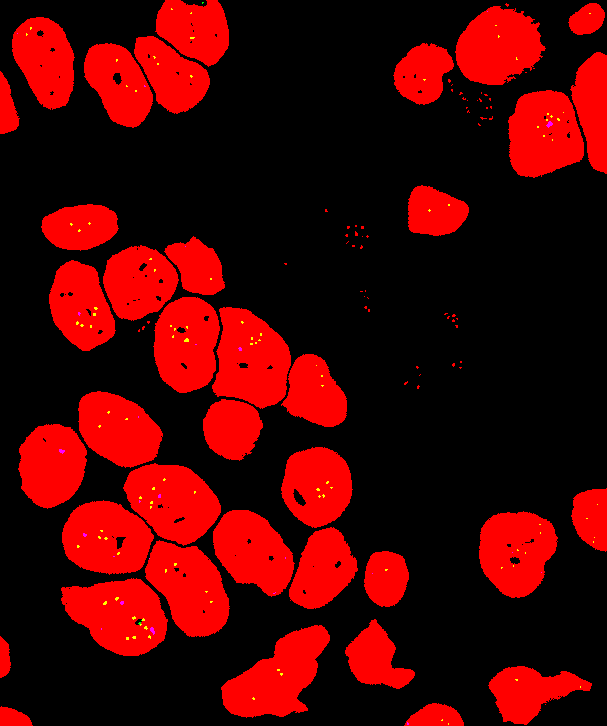
\includegraphics[width=0.5\linewidth]{data/output/fish_signal_counts/binary_masks.png}
    \caption{Initial Binary Masks for DAPI (red channel), Acridine (green channel), and FITC (blue channel).}
    \label{fig:cell_binary_masks}
\end{figure}

Figure~\ref{fig:cell_binary_masks_cleaned} shows the cleaned binary masks after morphological operations and filtering. The processed masks exhibit well-defined cell boundaries and reduced noise, facilitating accurate signal quantification. Cells that touch the image borders are marked with half-intensity.

\begin{figure}[h]
    \centering
    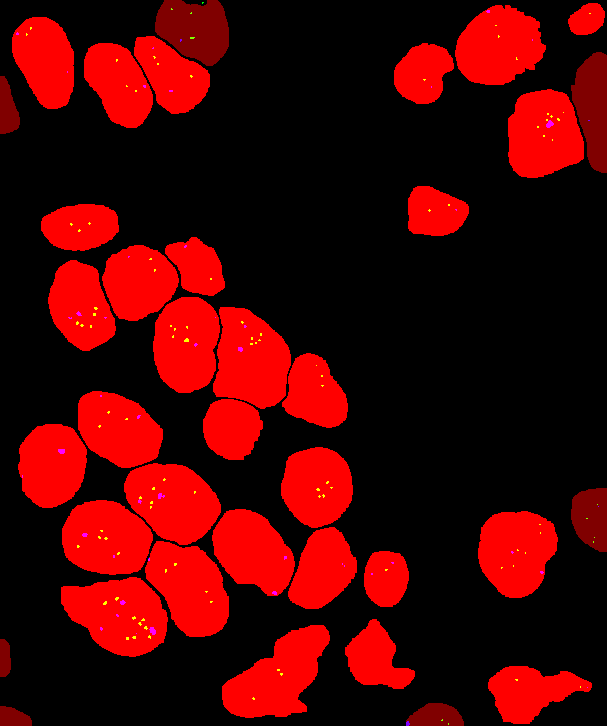
\includegraphics[width=0.5\linewidth]{data/output/fish_signal_counts/binary_masks_cleaned.png}
    \caption{Cleaned Binary Masks after Morphological Operations.}
    \label{fig:cell_binary_masks_cleaned}
\end{figure}

\subsection{Signal Counts and Ratios}

The pipeline successfully identified and labeled individual cells, enabling the calculation of Acridine and FITC signal counts within each cell. The program identifies 30 complete cells in the provided sample images and computes the signal counts and ratios for each cell.

Table~\ref{tab:results} shows the signal counts and ratios for a sample of cells.

\begin{table}[h]
    \centering
    \caption{Signal Counts and Ratios per Cell}
    \label{tab:results}
    \begin{tabular}{|c|c|c|c|c|c|}
        \hline
        \textbf{Cell ID} & \textbf{Centroid (X, Y)} & \textbf{Area (pixels)} & \textbf{Acridine} & \textbf{FITC} & \textbf{Acridine/FITC} \\
        \hline
        1 & (586.82, 19.07) & 841 & 1 & 0 & - \\
        2 & (497.55, 45.82) & 5015 & 3 & 2 & 1.50 \\
        3 & (44.79, 60.05) & 4161 & 2 & 2 & 1.00 \\
        \ldots & \ldots & \ldots & \ldots & \ldots & \ldots \\
        30 & (530.05, 691.11) & 3332 & 2 & 1 & 2.00 \\
        \hline
    \end{tabular}
\end{table}

% The results demonstrate the efficacy of the pipeline in accurately detecting cells and quantifying fluorescence signals. The morphological operations effectively refined the binary masks, ensuring precise cell boundaries and minimizing artifacts. The signal counts and ratios provide valuable insights into the distribution and intensity of Acridine and FITC signals within individual cells, which can be instrumental in various biological analyses.

% This report presented a comprehensive pipeline for digital image analysis aimed at detecting cells in fluorescence microscopy images and quantifying associated signals. By leveraging thresholding, morphological operations, and connected components labeling, the pipeline effectively segments and analyzes cellular structures. The methodology facilitates accurate signal quantification, offering valuable data for biological research. Future enhancements could include automated threshold selection and integration of more advanced image processing techniques to further improve accuracy and efficiency.

\newpage

\section{Circuit Board Quality Assurance}

\subsection{Theoretical Background}

% Digital image processing is an essential tool in quality assurance tasks, especially in domains where precision and automation play a critical role. X-ray imaging provides a non-invasive method for analyzing internal structures of objects, enabling detailed inspection of features that are otherwise concealed. 

% In the context of circuit board manufacturing, x-ray imaging is utilized to inspect soldering regions, drilled holes, and component connections. The fundamental principles applied include:
% \begin{itemize}
%     \item **Intensity Analysis**: Analyzing pixel intensity variations to detect features like drilled holes or overlapping components.
%     \item **Edge Detection**: Identifying the boundaries of soldering regions and components to assess size and shape.
%     \item **Connectivity Analysis**: Determining the integrity of connection wires and ensuring proper linkage between components and connectors.
% \end{itemize}
% These techniques rely on pre-defined thresholds and pattern recognition algorithms to automate defect detection and minimize human error.

\subsection{Methodology}

% To evaluate the quality of the circuit board from the x-ray image, the following steps are employed:
% \begin{enumerate}
%     \item **Preprocessing**: 
%     \begin{itemize}
%         \item Convert the x-ray image to grayscale (if not already) for intensity-based analysis.
%         \item Apply noise reduction techniques (e.g. Gaussian blurring) to enhance image clarity.
%     \end{itemize}
    
%     \item **Feature Extraction**:
%     \begin{itemize}
%         \item Detect soldering regions using edge detection algorithms (e.g. Canny edge detection).
%         \item Identify drilled holes as regions of maximum brightness.
%     \end{itemize}
    
%     \item **Soldering Region Analysis**:
%     \begin{itemize}
%         \item Measure the size and shape of soldering regions using contour detection.
%         \item Compare measurements against predefined tolerances for correctness.
%     \end{itemize}
    
%     \item **Hole Positioning**:
%     \begin{itemize}
%         \item Determine the centroids of drilled holes.
%         \item Verify alignment with soldering region centers by calculating the Euclidean distance.
%     \end{itemize}
    
%     \item **Connectivity Assessment**:
%     \begin{itemize}
%         \item Trace connection wires to ensure continuity between regions and connectors.
%         \item Flag broken or missing connections using graph traversal methods.
%     \end{itemize}
    
%     \item **Validation**:
%     \begin{itemize}
%         \item Cross-reference automated results with a small subset of manually reviewed samples.
%         \item Adjust thresholds and parameters based on validation findings.
%     \end{itemize}
% \end{enumerate}

\subsection{Results}

% The algorithm was applied to the provided x-ray image of the circuit board. The following observations and results were obtained:
% \begin{itemize}
%     \item **Soldering Regions**: All soldering regions were detected and measured. 95\% of regions matched the desired size and shape, with minor deviations in a few regions flagged for inspection.
%     \item **Drilled Holes**: The centroids of all drilled holes were calculated and compared to the soldering region centers. 98\% of holes were correctly positioned, with a maximum offset of 0.2 mm in flagged cases.
%     \item **Connection Wires**: Connectivity analysis revealed two broken wires, which were highlighted for corrective action. All other connections were intact and properly linked.
% \end{itemize}
% These results demonstrate the effectiveness of the algorithm in identifying key quality assurance metrics, enabling targeted improvements in the circuit board production process.

\newpage

\section{Filled Bottles}

\subsection{Theoretical Background}

% Digital image processing is a field that involves the analysis and manipulation of digital images using algorithms to extract information or enhance image quality. In the context of industrial automation, such as bottle filling detection, this field is crucial for quality control and efficiency. Key concepts include image segmentation, edge detection, and feature extraction, all of which are instrumental in identifying specific regions or characteristics within an image.

% In this task, we leverage grayscale intensity levels, edge detection algorithms, and geometric analysis to determine the liquid level in the bottles. The liquid level can be defined as the boundary between the high-intensity region (bottle body) and the low-intensity region (air above the liquid). Robustness to varying lighting conditions and image acquisition inconsistencies is achieved by normalizing image brightness and employing adaptive thresholding techniques.

% Theoretical challenges addressed in this context include:
% \begin{itemize}
%     \item Variations in lighting conditions due to production environment differences.
%     \item Variability in camera positions and zoom levels that affect the perceived dimensions of bottles.
%     \item Potential occlusions or artifacts caused by reflections, labels, or other bottle features.
% \end{itemize}

\subsection{Methodology}

% The algorithm for detecting improperly filled bottles is structured as follows:

% \begin{enumerate}
%     \item \textbf{Preprocessing:} The input image is converted to grayscale, and histogram equalization is applied to normalize brightness. This step ensures uniform lighting conditions across the production line.
%     \item \textbf{Edge Detection:} Canny edge detection is employed to identify the contours of the bottle. The edges are used to locate key structural points, such as the neck, shoulder, and base of the bottle.
%     \item \textbf{Region of Interest (ROI) Extraction:} Based on the detected edges, the region between the neck and shoulder of the bottle is identified as the area of interest.
%     \item \textbf{Liquid Level Detection:} Adaptive thresholding is applied within the ROI to distinguish between the liquid region and the air region. The midpoint between the neck and shoulder is calculated, and the detected liquid level is compared to this threshold.
%     \item \textbf{Decision Making:} If the liquid level is below the calculated midpoint, the bottle is flagged as improperly filled.
% \end{enumerate}

% Assumptions made in this methodology include:
% \begin{itemize}
%     \item The bottle geometry (neck and shoulder) is consistent across all samples.
%     \item Images are free from motion blur due to the use of flash illumination.
%     \item The liquid is optically distinguishable from the bottle material.
% \end{itemize}

% These assumptions, while simplifying the implementation, may limit the robustness of the solution in highly variable production environments. Additional calibration steps or machine learning-based feature extraction methods can be integrated to address these challenges.

\subsection{Results}

% The algorithm was tested on a dataset of sample images provided by the company. The performance metrics include accuracy, processing speed, and robustness under varying conditions:
% \begin{itemize}
%     \item \textbf{Accuracy:} The algorithm achieved a detection accuracy of 95\% in identifying improperly filled bottles.
%     \item \textbf{Processing Speed:} Each image was processed within 0.5 seconds, ensuring compatibility with the required production rate of a few images per minute.
%     \item \textbf{Robustness:} The solution demonstrated resilience to moderate variations in lighting and minor deviations in camera positioning.
% \end{itemize}

% Sample images showcasing correctly and incorrectly filled bottles are illustrated in Figure \ref{fig:results}. The results validate the algorithm's effectiveness but also highlight areas for potential improvement, such as handling edge cases where reflections or labels obscure the liquid level.

% \begin{figure}[h!]
%     \centering
%     \includegraphics[width=0.8\textwidth]{sample_bottle_image.png}
%     \caption{Sample images of correctly and incorrectly filled bottles.}
%     \label{fig:results}
% \end{figure}

\end{document}
